
\section{Background}\label{sec:background}
%
%\subsection{Curriculum Reform}
%As previously mentioned, CS curricula are being reformed globally.
%
%





\subsection{Computational Thinking}

There is no general consensus on the definition of Computational Thinking (Yadav, 2015). Voogt et al (2015) call for a flexible and pragmatic approach and use operationalization of CT, such as has been done by Yadav (2015). Computational Thinking refers to thought processes that are involved when solving complex problems and generalizing and transferring this problem solving process to a wide variety of problems (Voogt et al 2015). CT are higher-order-thinking skills  (Yadav2017 CT for educators) and considered an extension of every child's analytical ability (Wing 2006)(Voogt et al 2015).


Wing (2006) identifies the following CT skills:\label{CTdefWing}
\begin{itemize}
\item Algorithmic Thinking: thinking in terms of rules, steps and repetitions (of subtasks
\item Decomposition: Breaking a problem into sub-problems (which can be dealt with individually)
\item Abstraction: simplifying a problem by leaving out (unnecessary) details
\item Generalization: finding patterns and re-using solutions (transfer)
\item Evaluation: Does my solution solve the problem? Analysis: How could process/solution have been improved?
\end{itemize}





Several studies report an evident link between programming and CT (Davies, 2008)(Hu, 2011)(Crick, 2017)(Yadav et al., 2017).


%In a survey of program understanding, von Mayrhauser and Vans
%(1994) summarise studies (in particular Guindon, 1990) noting that experts:
%have efficiently organised and specialised knowledge schemas; organise their
%knowledge according to functional characteristics such as the nature of the
%underlying algorithm (rather than superficial details such as language syntax);
%use both general problem solving strategies (such as divide-and-conquer) and
%specialised strategies; use specialised schemas and a top-down, breadth-first
%approach to efficiently decompose and understand programs; and are flexible in their approach to program comprehension and their willingness to abandon
%questionable hypotheses.[Robins, Rountree, Rountre (2003).  ]


\subsection{Algorithms, Algorithmic Thinking, and Problem Solving}

Algorithms is a fundamental CS concept. Algorithms are tools for developing and expressing solutions to computational problems (Grover and Pea, 2013). To be successful in developing novel algorithms that solve problems correctly and successfully, calls for a coherent set of skills and knowledge.
On the one hand, algorithmic thinking (as part of CT) and problem-solving skills are essential (Lister et al, 2004). On the other, fundamental knowledge of the concepts of algorithms are needed, i.e., how algorithms work, which common algorithms and plans exist, and knowledge about strategies for composing (or combining) algorithmic components. CT thought processes are involved in formulating problems so their solutions can be represented as computational steps and algorithms (Aho, 2012). 

\note{CT learning takes place during programming (Brennan and Resnick, 2012)(Lye and Koh, 2014).}


\todo{How to develop skills and reinforce knowledge related to algorithms… either through concepts or programming. <SEE VERHAAL VAN DENNING, 2017>}


McCracken et al. (2001) describe five iterative steps to problem solving (abstracting, generating sub-problems, implementing sub-solutions, integrating sub-solutions, evaluating and iterating) and encompass the CT skills as defined by Wing (algorithmic thinking, abstraction, decomposition, generalization, evaluation) described by Wing (2006). The step of integrating sub-solutions (via abutment, merging and nesting) corresponds with algorithmic thinking, as it includes involves creating an algorithm that controls the sequence of events. An important aspect of it's opposite step, generating sub-problems, is recognizing plans, existing methods or strategies. Recognizing plans at an abstract level helps decompose the problem and simplifying the problem. What is left behind is to fine-tune the plan to the specific situation and then integrate it with the remaining sub-solutions.


\subsection{Assessment best practices}

A substantial amount of research has been done to role of assessment in education. In his study Frederiksen (1984) describe assessment as a motivator for learning. Alderson and Wall (1993) and Prodromou (1996) elaborate by stating that what is assessed strongly influences what is learned. Biggs (1996) prescribes that instruction, learning and assessment must be well-aligned. This alignment exists in most traditional knowledge-based tests, yet constructive alignment for competency-based instruction is not self-evident (2006Baartman). With the emphasis of Computational Thinking and problem solving in reformed CS curricula, learning and instruction is increasingly competency-based. Assessment of competencies is complex, mainly because it comprises a multi-facetted blend of knowledge, skills and attitudes (Van Merriënboer, Van der Klink and Hendriks, 2002).

\subsubsection*{Assessment Criteria}\label{sec:qualityCriteria}
Baartman et. al. (2006) proposes a 'wheel of competency assessment' framework of quality criteria for competency assessments which integrates different assessment methods into a Competency Assessment Programme (CAP). It constitutes both fit-for-purpose quality criteria (i.e. alignment, transparency, authenticity, \ldots) as well as fit-for-use utility criteria (i.e. cost and efficiency). The framework has been extended by Catete (2017) with classical psychometric quality criteria of validity and reliability. This adapted framework has recently successfully been applied to establish quality-assured programming rubrics for AP CS Principles (2017Catete).
\note{2017Catete geeft een mooi overzicht van de aspecten van de wheel, pg 100} Yadav (2015) expresses availability and ease of access an additional feature.




\subsubsection*{Design methods}

In his work, Hermansen (2014) suggests that teachers should work collaboratively on transforming (rather than implementing) assessment tasks. Such a development and refining process yields assessments specific to local settings, adhering to the needs, knowledge, skills and interests of their own students.

The Dutch curriculum description includes high-level goals (Barendsen et al. 2016). However, this description is not specific enough for the assessment. Concrete learning outcomes including the level of comprehension (taxonomy) need to be established. A similar situation exists in the UK national curriculum. The levels from the previous ICT curriculum have been removed, leaving assessment at KS3 to the responsibility of individual schools. CAS members (in co-operation with CAS Master teachers, teachers and academics) have taken the initiative to establish computing progression pathways and rubrics to assess learners' Problem-solving and Computational Thinking capabilities. With it, learning objectives and potential evidence observations have been established, yet seems to miss concrete alignment with potential works products. Importantly, Giordano (2015) concludes that designing questions clearly linked to the competencies is perceived as the most difficult task in the assessment process. Moreover, the more authentic and realistic, the more complex the detailed mapping to the abilities/competenties becomes. These is very relevant as the curriculum specifies a concept-context approach to learning. This authentic learning approach encourages students to connect real world problems to the subject matter at hand. In their paper, Goode (2014) emphasize why this makes sense: "engaging students in the context of complex, meaningful projects that require sustained engagement, critical thinking, collaboration, management, communication, and management of resources to develop final products or presentations builds the types of 21st century skills advocated by new sets of national standards". Especially when dealing with more complex tasks, explicit alignment between learning objectives, observations and work products must be established.

%\subsubsection*{Learning objectives and FKSAs}
\todo{ Naar achtergrond met meer toelichting, uitleggen. What is abilities (niet attitutes?)? What is verschil tussen skill en abilities?}
\todo{Why needed}


\note{knowledge, skills or other attributes}
%
%linked to evidence-eliciting-performances



\textbf{Evidence-Centered Design}\newline
Initiatives in the U.S. follow a different, rather structured, path, incorporating validity evidence into an assessment design process. SRI launched a Teacher Assessment Literacy for Exploring Computer Science study to investigate the design and delivery of high-quality assessment literacy materials. They use an Evidence-Centered Design (ECD) method. ECD is a principled method for modeling domains for assessment purposes that is especially useful for hard-to-assess practices (Grover, 2016). Its systematic structure facilitates a coherent mapping from high-level curricular goals to observable behaviors. This yields three models which elicit evidence of students' achievement levels of learning objectives. The student model specifies the knowledge, skills or other attributes (KSA) to be assessed. The evidence model describes observable behaviors or performances which may provide evidence about the knowledge or skills to be measured, and thus links the chain of reasoning from
students’ performances to their knowledge and skill. The task model describes ways to elicit data that provide evidence about student. Evidence is obtained by deliberately putting students in those situations, challenges, or tasks that will elicit the desired FKSAs (Grover and Bienkowski, forthcoming).






\note{Evidence models
lay out the argument about why and how observations in a given task
situation constitute evidence about student model variables. There are
two parts to an evidence model, the evaluation component and the
measurement component.}

This methodology has been used by, extensively reported on, and cited to by Mislevy et. al. (2002, 2003). It has recently also been in CS used by Grover (2017), Snow (2017), and for the development of assessment instruments for the Exploring Computer Science curriculum, as described by Mislevy (2006) and McGee (2018)\todo{[2018McGee CS outcomes]}.



\begin{figure*}\label{fig:ECD}
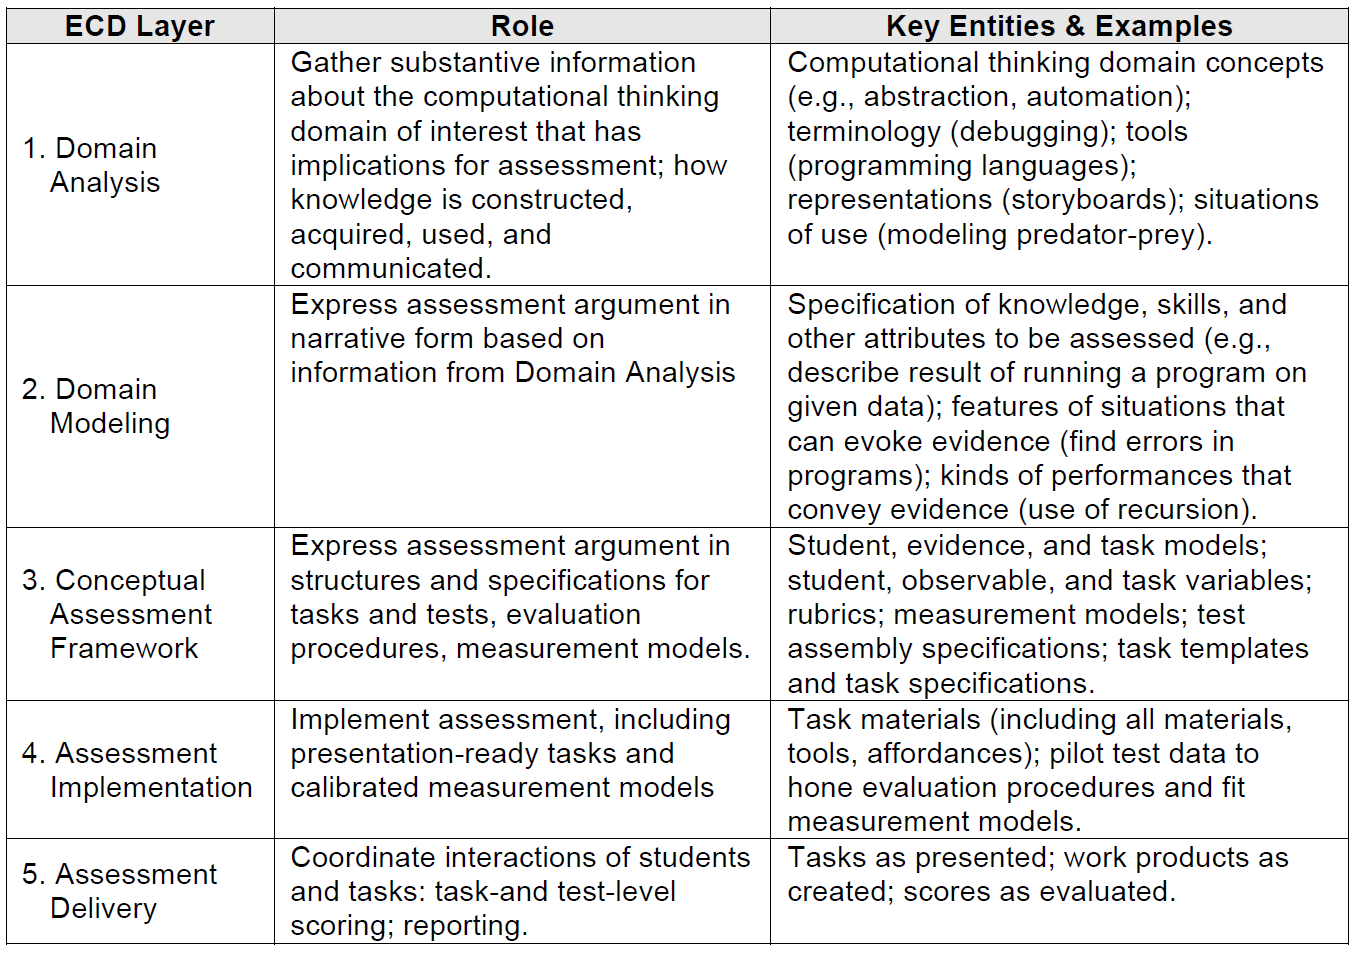
\includegraphics[scale=0.6]{figures/ECDoverview.png}
\caption{Roles and Key Entities in the Five Layers of Evidence-Centered Design (2014SnowBienkowski)}
\end{figure*}



%\begin{itemize}
%\item \textbf{Domain Analysis:}
%The top layer in the ECD process is a Domain Analysis to clarify learning goals.
%This level includes determining relevant concepts and terminology,(e.g. abstraction, algorithms), tools (i.e. programming languages) and representations (flowcharts, pseudocode) as well as understanding how knowledge is constructed, acquired, used and communicated (SRI Assessment Design Patterns for CT, 2017). In the process, the curricular learning objectives are translated into more specific and learning goals specified in operational terms, ready for teacher use
%\item \textbf{Domain Modelling:} the assessment argument was designed. The learning goals were translated into the specific focal knowledge, skills, and attributes (FKSAs)
%
%\item \textbf{Conceptual Assessment Framework:}
%The result of this phase was a design pattern consisting of three aligned models (student model, evidence model, and task model) which together form the assessment specifications: the foundation for the new assessment.
%
%\item \textbf{Assessment Implementation:}During the implementation stage, the model assessment tasks are translated into classroom-specific assessment tasks in the designated programming language.
%
%\item \textbf{Assessment Delivery:} the tasks are administered to students.
%\end{itemize}


Transitioning from one ECD layer to the next involves analytical precision and careful reasoning. To validate this step, Catete (2017) uses an expert panel. Several methods can be used to resolve any differences in opinions and obtain an object consensus between panel members, such as focus groups\todo{ref WIPSCE artikel over thresholds}, Nominal Group Technique\todo{Adler, M. & Ziglio, E. Gazing into the oracle: The Delphi method and its application to social policy and public health. Jessica Kingsley Publishers, 1996.} or the Delphi method\todo{ref brooks 779}.




\todo{Methode geven om meningsverschillen plat te strijken.  DELPHI?? De moeite waard? Misschien delen van DELPHI methode gebruiken? Kijk evt naar artikel over thresholds WIPSCE, evt met een focusgroep (is sneller en minder zwaar aangezet). Beschrijf hier hoe je verschillen gaat oplossen. Relateer evt ook aan ECS ECD met DELPHI. Elementen van methode gebruiken, niet hele methode, Nominal Group Technique? (zie 2017 catete.}





\subsubsection*{Taxonomies}

Taxonomies can be used to provide a language for describing learning outcomes and
performance in assessments, dividing them into domains (such as cognitive, affective, and psychomotor) or categories based on complexity of the task. Two widely used taxonomies for assessment of learning are the (revised) Bloom
taxonomy and the SOLO taxonomy. Both have been used in CS education research (revised Bloom: Whalley et al., 2006 and SOLO: Lister et.al 2006).


However, it has been reported that there are some drawbacks to their use in CS. Thompson et. al. (2008) report that experts have difficulties applying Bloom's taxonomy consistently in introductory programming courses. The classification becomes meaningless as all tasks seem to fall into the same category. Given the difficulties in categorizing programming activities within the existing taxonomies, several attempts have been made to propose new taxonomies appropriate for CS education.

\note{In part this is because the terms synthesis and evaluation are not useful in describing programming learning outcomes.} Fuller et. al. (2007) explain that though SOLO can be used for holistic marking, it says nothing about the type cognitive processing, such as recalling items or drawing conclusions. They suggest to separate Bloom’s levels into two dimensions, producing (writing) and interpreting. Lister and Leaney (2003) attempt to differentiate in terms of magnitude of the code.

Meerbaum-Salant et. al. (2013) propose a hierarchical taxonomy scale describing how student’s performance grows in complexity. It’s aim is to pinpoint (the development of) programming skills: both problem solving (such as plan composition) and (construct-based) language aspects. It is based on a combination of the Revised Bloom and Solo taxonomies. The result is a nine-level taxonomy with
the highest level being relational creating, and the lowest level being
unistructural understanding (on one axis: understanding, applying, creating; on the other: unistructural, multistructural, relational)\todo{ Erik: Laat de lezer de taxonomieen zien, evt met figuren (wat meer toelichten)
}:


%Meerbaum-Salant et. al. (2013) propose a hierarchical taxonomy
%scale based on a combination of the revised Bloom and Solo taxonomies
%\cite{Meerbaum2013}. Three super-categories - unistructural, multistructural,
%and relational (derived from the Solo taxonomy) were chosen, each containing
%three sub-categories - understanding, applying, and creating (derived from
%the revised Bloom's taxonomy:

\begin{description}[leftmargin=1em]
\item[Understanding:] The ability to summarize, explain, exemplify,
    classify, and compare CS concepts, including programming constructs.
\item[Applying:] The ability to execute programs or algorithms, to track
    them, and to recognize their goals.
\item[Creating:] The ability to plan and produce programs or algorithms
    (constructing, analysing, evaluating and formulating).
\item[Unistructural:] The ability to create very small scripts doing one
    thing, or adding an instruction with a local effect to an existing
    script.
\item[Multistructural:] The ability to track a program and grasp various
    parts but not the entity they form as a whole.
\item[Relational:] The ability to fully understand a complex concept (such
    as concurrency) and to coherently explain its various facets.
\end{description}






\subsubsection*{Identifying levels of mastery}
A substantial body of work has previously explored the assessments used in novice programming courses in tertiary education (Luxton-Reilly, 2018)\todo{mer woorden gebruiken, uitleg vanuit docenten stoel}. In prior work, researchers claimed that the subject itself was difficult. McCracken et al. (2001) discuss how students fail to complete tasks, and Robins, Rountree, Rountre (2003) associate it with high dropout rates in introductory programming courses.  However, more recently, assessment tasks were found to be more complex than academics expected (Whalley, Lister et al., 2006; Luxton-Reilly, 2018)\todo{geen twee refs achter elkaar}. For example, tasks typically require both algorithmic thinking (initialize before changing), as well as a more advanced understanding of data representation (assigning a value to a property)(Seiter, 2013).

Assessment tasks should adequately indicate a students’ programming comprehension and clearly discriminate between achieved performance levels. Predicting the difficulty of programming tasks and understanding alternative conceptions has shown to be difficult (Lonati, 2017)\todo{ Toelichten: bv een invulopgave kan op verschillende manieren aangepakt worden}. In their findings, Oliver et al., (2004) indicate that introductory and intermediate programming courses assess at a constant level of difficulty and restricted solely to Bloom’s application and analysis level. The inability to accurately measure student performance may well contribute more to the poor results highlighted in several studies (such as the McCracken et al, 2001) than failures of student comprehension [2010TewGuzdial].  In their paper, Whalley et al. (2006) also relate the high failure rate in introductory programming courses to unfair and inappropriate assessment instruments, especially for non-elite institutions.




However, whatever taxonomy chosen, scientists agree that classifying tasks is far from straightforward (Fuller et al., 2007; Thompson, Luxton-Reilly, Whalley, Hu, and Robbins, 2008). As a result, researchers exclaim that "the pattern of achievement is not clear" (2013Zur-Bargury), making their analysis difficult and inconclusive. Maybe the issue is not the taxonomy, but rather the task being classified.

In their research Luxton-Reilly (2018) state that “most assessments used in formal examinations combine numerous heterogeneous concepts, resulting in complex and difficult tasks”. We agree that difficulty that experts endure whilst trying to classify the tasks (Meerbaum-Salant et al, 2013) is related specifically to the nature of the tasks. De Raadt et al. (2009) explains that the identification, selection and application of plans which can be seen as a representation for strategy (similarly described by Soloway (1985), also known as patterns (Wallingford, 1996)). They distinguish a set of elementary plans (programming strategies) that can be combined to create a solution. Soloway (p. 856) and de Raadt identify the following methods of integrating plans (bottom-up):
-	Abutment: plans following each other in sequence. For example, initializing a variable and printing it’s value (i.e. x=12; print(“The value of x is: “, + str(x) ) )
-	Nesting: one plan as a whole is submerged in another. For example, printing the value of a variable is constituent to a counting plan.(i.e. counter=0; while not done counter ++;print(“The number of items is: ” + str(counter)) )
-	Merging: interleaving (at least) two plans. For example, in the averaging problem, the input, summing and counting plans are merged.


Examples are Initialization plan (variables), Average plan, Triangular Swap plan, Guarded Division plan, Counter-Controlled Loop plan, Sum and Count plans, Bubble Sort algorithm.

Strategies can be expressed both simply, at a sub-algorithmic level, and at a higher level which are found in solutions produced by expert programs (de Raadt, Toleman and Watson, 2006). A number of attempts have been made to decompose these strategies (Muller, Haberman, and Ginat, 2007; Porter and Calder, 2003; Wallingford, 2007) \todo{ Erik: uitsplitsen en toelichten wat ieder gedaan heeft zodat je dit als lezer niet zelf hoeft op te zoeken }into  smaller units and distinguish pre-requisite knowledge. These plans and higher level algorithms map to multi-structural and relational levels in the SOLO taxonomy. In their combined efforts, Luxton-Reilly et al. (2018) have managed a first step towards decomposition, by for example recognizing and identifying initialization, use of conditionals and nesting.  \todo{ Erik: Zhong hier relevant over task?}




Cross-referencing, we see that Luxton-Reilly et al.’s top-down approach in which they decompose a complex task does not systematically consider all concept combinations and thus sources of difficulties and alternative conceptions. For example, in their nesting-task, they fail to recognize \todo{nuanceren}that a student may not understand the difference between a loop nested in a conditional and a conditional nested in a loop. De Raadt et al. is also not complete, missing the idea of procedures, functions, parameters, and a Boolean-Flag loop plan as a specific form of a primed sentinel controlled loop plan. Here too we see that underlying concepts at a unistructural level are left out\todo{nuanceren}. For  example the very first plan, the average plan, explicitly states the need to understand the division operator, but not the assignment of variables .

In his work, Lister (2010, 2016) positions the Piagetian and neo-Piagetian theories. The Piagetian theory describes how students may reside in different stages of cognitive development for each fundamental concept being taught. The neo-Piagetian theory extends this with the idea with an ”overlapping waves” model, a novice programmer can reside in multiple stages simultaneously. The stages coincide with those of the SOLO taxonomy. In their paper, Szabo et al. (2014) propose a curriculum analysis methodology based on Neo-Piagetian theory to facilitate lecturers in tracing the development and assessment of concepts throughout their courses. This theory describes how students may reside in a different stages of cognitive development for each fundamental concept being taught. CAS has developed Computing Progression Pathways (Dorling and Walker, 2014) to identify the major knowledge areas (concepts) and CT skills of computing and provides specific indicators of increasing levels of mastery (e.g. distinguishing between ‘understands’ and ‘can apply’) of the subject in those areas (Giordano, 2015  ).\todo{ Erik: Licht toe en zet tegen elkaar af: “de ene onderzoek maakt wel onderscheid tussen verschillende… maar niet…”} \todo{ Nesten is een complexiteit op zichzelf
“Afhankelijkheid is geen onderdeel van de onderzoek van… “}

Summarizing, the introduction of the new computing curriculum could benefit from tooling which aids the establishment of assessments. Teachers will and should create assessments tailored specifically to their classroom needs, but lack specific PCK to do so. Not only is creating a qualitative assessment acknowledged as a difficult task, in this particular case, teachers must first acquire and internalize knowledge about the new concepts and may not yet have reached the desired final level.





\subsection{Assessment Techniques}
Assessments are used for several purposes. McMillan (2007) distinguishes between two types of assessments, summative and formative. Summative assessment refers to the use of assessment-based evidence to help us arrive at go/no-go decisions based on the success of a completed course or instructional program (Popham, 2009). On the other hand, assessment for learning is formative. Formative assessment is used by both students and teachers to adjust ongoing instructional and learning activities in order to improve the manner in which learning is taking place. Summative assessment can also be treated formatively, for example to determine the effectiveness of instruction.


\subsubsection*{PCK}

Effective teaching requires a combination of pedagogy, content, and knowledge (PCK) (Shulman, 1986). In a nutshell, it means that subject matter (content knowledge) and ways of teaching (pedagogical knowledge)(Yadav, 2016) are integrated. It encompasses about knowing what makes certain topics easy or difficult, as well as ways of representing and formulating topics in different ways (Shulman, 1986).

Magnusson, Krajcik en Borko (1999) distinguish four aspects of content-specific PCK: knowledge of
(1) curricula, (2) students' understanding and difficulties, (3) instructional strategies, and (4) assessment.


In this research we focus on one aspect of PCK, namely assessment. \todo{and are particularly interested in the PCK aspects needed to adapt and implement particular types of assessment}


\subsubsection*{Assessment as a part of PCK}
Very little is known about PCK for Computing (Yadav, 2016). As a part of PCK, teachers have limited knowledge about assessment and seriously struggle with it (Popham, 2009). Particularly, teachers face many challenges with respect to the assessment of new topics (DeLuca and Klinger, 2010). The 2015 study by Computer Science Teacher's Association (CSTA) found that teachers face a number of challenges finding valid and reliable assessments to use in their classrooms. Along the same line, Dutch teachers say they lack qualitative (peer-)reviewed materials, assessment rubrics and question banks (Tolboom et al., 2014). Yadav et al. (2015) conclude that teachers lack PCK, which manifests itself in an incapacity to act: teachers understand need for qualitative assessment, but just don't know how to.

%Both experienced and novice teachers struggle in assessing student learning (Fincher, Kolling, Utting, %Brown, Stevens 2010)(Hebert \& Worthy, 2001)(Veenman, 1984) (Yadav, 2016)(Yadav, %2015)(Bardensen et al., 2015 ITICSE wg).

Faced with a specific assessment task, teachers generally take previously developed templates as a point of departure and adapt them to meet their current requirements (Hermansen, 2014). During his observations he saw that teachers spent significant time on aspects related to eliciting evidence of students' approach to a task. This indicates that teachers are well-informed about the role of an assessment.
Particularly, teachers face many challenges with respect to the assessment of new topics (DeLuca \&Klinger, 2010). The 2015 study by Computer Science Teacher's Association (CSTA) found that teachers face a number of challenges finding valid and reliable assessments to use in their classrooms. Along the same line, Dutch teachers say they lack qualitative (peer-)reviewed materials, assessment rubrics and question banks (Tolboom et al., 2014). Yadav et al. (2015) conclude that teachers lack PCK, which manifests itself in an incapacity to act: teachers understand need for qualitative assessment, but just don't know how to. To elicit: CS teachers assess merely a small spectrum of levels in Bloom's taxonomy, ascertained by Oliver et al. (2004) and confirmed by Whalley et al. (2006). Depending on the particular concept, in some cases only the lower knowledge levels are assessed (networks), in others predominantly the higher application and analysis levels (programming). Either way, this leads to non-discriminative assessments. Even if there is published material available, many teachers create and rely on their own material (Popham, 2009).

Thus, judgements about students' proficiency are made without the use of validated assessments. If the quality of assessment is insufficient, the teaching will be ineffective (Ragonis, 2012).  If teachers use low-quality assessment instruments we will end-up teaching the wrong subject; and vice-versa (Giordano et al., 2015).  Whalley et al., (2006) describe the assessment of programming as complex and challenging and emphasize the lack of clear frameworks and tools.





In his review on developing generic resources for assessment, Hermansen (2014) concludes, based on several researches (Coburn, 2001, 2003; Edwards, 2008; Horn \& Little, 2010; Hutchinson \& Hayward, 2005; Rasmussen \& Ludvigsen, 2009; Tierney, 2006), that assessment tools aren't plug-and-play modules that remain instantaneously operable after a relocation. Rather, they must be adapted  and 'recontextualized' according to classroom needs. From his review he summarizes that teachers who implement formative assessment resources "draw upon a strong understanding of subject knowledge, use a range of ideas and tools to enable classroom interaction and learning, have established a new division of labour in their classrooms, focus on developing student learning and autonomy, and critically examine their own beliefs about learning and classroom practices" (Black \& Wiliam, 2006; Brookhart, Moss, \& Long, 2010; Harrison, 2005; James \& Pedder, 2006; MacPhail \& Halbert, 2010; Suurtamm et al., 2010; Webb \& Jones, 2009; Willis, 2011). This list alone affirms that any teacher new to a particular concept, or new at all to teaching, will likely be lacking some, if not all of these skills or knowledge.


Teacher educators need to provide teachers with the content, pedagogy, and instructional strategies needed to incorporate computational thinking, and in particular the assessment of the its core concepts (Yadav2017).



\subsubsection*{CT assessment}
With the lack of a precise definition as one of its contributing factors, Computational Thinking is perceived to be one of the more challenging concepts to teach and assess (2017Crick).

There is no clear definition of CT(Crick, 2017) making it difficult to assess. Recently some research into assessment of Computational Thinking has been published (Yadav, 2017)(Yadav, 2016). Evaluating CT is perceived as difficult (Brennan and Resnick, 2012) (Crick, 2017).
Without rigorous assessment, computational thinking cannot be successfully embedded in education (Grover et al., 2014).

Grover et. al. (2017) call for measures that enable educators to assess student learning of CT.  Specifically they signal the necessity to test and validate materials in various settings with diverse learners.
Assessments of CT remain underdeveloped and under-researched (Yadav et al., 2015).
Educators need a manner to assess and validate what CT a student has learned (Grover and Pea, 2013).
In their review study, [2014LyeKoh], summarize that of the research on computational thinking through programming , stunningly none focus on upper secondary high school (ages 15-18) (but merely on elementary or higher education).


\subsubsection*{Algorithms assessment}
Poor CS1 results: Lister, McCracken


The 2001 ITiCSE report by the McCracken Group (McCracken, 2001), a keystone in assessment literature (Giordano, 2015) on CS concepts, describes the difficulties pertaining to the development and validation of assessment activities. They raise concerns about task selection and the difficulties of standardizing assessments for multiple institutes.

\subsubsection*{Fit-for-purpose assessment tasks}
CS1 much research to assessment tasks: mc, parsons, sniplets,


meet the criteria in \ref{sec:qualityCriteria} in addition

\subsection{Black hole: Assessment in Secondary CS education}
There is a gap between the (lean) research and classroom practice (Yadav, 2015). All-in-all, little research has been done on the effectiveness of the assessment materials available (Yadav,2016). Computing education and research suffer from the lack of assessment instruments (Voogt et al., 2017). In their research [2010TewGuzdial], argument the importance of validated assessment that could be widely applicable across tertiary curricular approaches. This may be even more true for secondary education, where far less relevant research has been done in the first place. In addition, research developments are not accessible to teachers (either they need a paid subscription, academic literature may be written in an incomprehensible manner, or not practical as it can’t be implemented in the classroom in a cost-effective manner). Recent published work based on CT have a focus in primary education or middle school(review studie LyeKoh 2014). Research based on (the assessment of) CS concepts has a focus on tertiary education (such as McCracken 2001, TewGuzdial 2010). Merely a few studies focus on CS concepts or CT specifically in secondary education.



